\documentclass[../defence.tex]{subfiles}
\begin{document}

  \begin{frame}{Bischichtiges Graphen auf Metallsubstraten}
    \begin{columns}[onlytextwidth, T]
      \column{\dimexpr\linewidth / 6 * 3}
        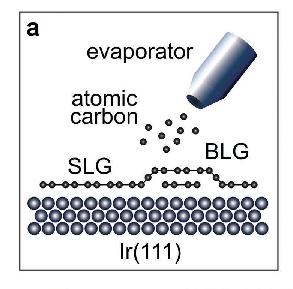
\includegraphics[width=\linewidth]{images/bilayer_production.pdf}
        \cite{sab2018}
      \column{\dimexpr\linewidth / 6 * 2}
        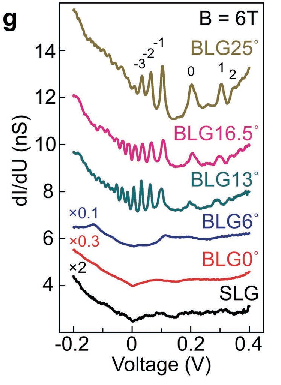
\includegraphics[width=\linewidth]{images/angle_dependence_bilayer.pdf}
        \cite{sab2018}
    \end{columns}
    \note{
    \begin{itemize}
      \item Monoschicht wird chemisch dampfabgelagert
      \item Zweite Schicht mit Druck untendrunter gebracht (obere Schicht bleibt erhalten wegen der hohen Bindungskräfte in der Ebene)
      \item Abhängig vom Drehwinkel zwischen den beiden Graphenschichten werden die Landauniveaus wieder sichtbar
    \end{itemize}
    }
  \end{frame}

\end{document}
